\documentclass[10pt,a4paper]{article}
\usepackage[utf8]{inputenc}
\usepackage[T1]{fontenc}
\usepackage{amsmath}
\usepackage{amsfonts}
\usepackage{amssymb}
\usepackage{graphicx}
%\usepackage{tikz}
\usepackage{float}
\usepackage{tikz-cd}

\newcommand{\ImageWidth}{11cm}
\usepackage{tikz}
\usetikzlibrary{decorations.pathreplacing,positioning, arrows.meta}

\usepackage[backend = biber, style=bwl-FU]{biblatex}
\addbibresource{bibliography.bib}

\usetikzlibrary{fit,positioning}

\author{}
\date{}
\title{Some notes on the state-space LBM}

\begin{document}
\maketitle


\begin{abstract}
	\noindent In response to the global coronavirus pandemic, we study co-clustering of multivariate time-series data as a way to simultaneously cluster both geographical regions and time periods after the outbreak of the pandemic. The resulting blocks of clusters, identified with a latent block model component, are integrated with an extended SIR model that takes both geographical clusters as well as clusters of time periods into account. We consider US data (or global or both?) and show how the novel latent block SIR model produce better prediction accuracy of the epidemic, and gives further understanding of how the virus is spreading in different geographical regions during different periods of time. 
\end{abstract}	

\section{Background}

The latent block model \parencite{govaert2003clustering} is a commonly used model for co-clustering of large data matrices. It is a model-based approach that assumes that the rows and columns of the data matrix can be arranged according to latent row and column clusters. It has been extended to cover the case of counting data \parencite{govaert2010latent}, continuous data \parencite{nadif2010model}, categorical data \parencite{keribin2015estimation}, ordinal data \parencite{jacques2018model, corneli2020co}, functional data \parencite{Bouveyron}  and tensor data \parencite{boutalbi2020tensor}. In this work, the latent block model is extended in two ways: first by covering time-series data of proportions, and secondly by being integrated with the SIR model \parencite{kermack1927contribution}, commonly used in the analysis of disease spread.

The class of SIR models are used to describe the spread of disease in a population. For a review of infective disease modeling, see \cite{keeling2011modeling}. Compartmental models such as the SIR model has been used for modeling of infective disease for more than a 100 years \parencite{ross1911some}, and have historically been used to e.g. understand disease transmission dynamics \parencite{mills2004transmissibility}. With the 2020 coronavirus pandemic, attention has been focused on forecasting. Special attention has been given to key outbreak measures like peak intensity and the timing of such intensity. With accurate estimates of these quantities, policy makers have the opportunity to make informed decisions on allocation of resources, implementation of interventions and communication to the public \parencite{chretien2014influenza, nsoesie2013forecasting}. For the simplest case of the SIR model, a population of susceptible cases $S(t)$ are exposed to a fraction $I(t)$ of the population that are infected at time point $t$. As a consequence, a part of the susceptible cases will be transferred to the group of removed cases, denoted $R(t)$. The removed cases consist of both recovered and dead cases, and once a case enter this group there is no possibility to enter the group of susceptible and infected again. Following from this definition, $S(t) + I(t) + R(t) = 1$ for all $t \in [0,T]$ and $S(t), I(t), R(t) > 0$. This dynamic system is described by the following differential equations: 
%
\begin{equation}\label{SIR}
	\frac{dS(t)}{dt} = -\rho S(t)I(t), \quad \frac{dI(t)}{dt} = \rho S(t)I(t) - \gamma I(t), \quad \frac{dR(t)}{dt} = \gamma I(t),
\end{equation}
%
where $\rho > 0$ is the transmission rate of the disease, and $\gamma > 0$ is the rate of recovery. The model in (\ref{SIR}) describes the transport of cases between the three groups of susceptible, infected and removed individuals. It is therefore often called a compartmental model \parencite{ramsay2017dynamic}. Note that although the transmission rate $\rho$ is constant, the rate of transport between the group of susceptible and infected cases does depend on time since the number of susceptible cases decreases as the number of infected increases. This follows from the fact that the total group of susceptible, infected and removed cases at all times equals the total population. Note also that the SIR model implicitly assumes that the cases are mixed freely with the entire population \parencite{ramsay2017dynamic}.

\section{The Extended SIR Model}
Compartmental models like the SIR model are purely deterministic, but recently, several probabilistic versions of such models have been suggested. One of the most recent proposals is given in \cite{osthus2017forecasting}, where a state-space model motivated by the SIR model is presented, where inference and forecasting is conducted under a Bayesian setting. In \cite{song2020epidemiological}, the model was extended to cover multivariate time-series, and a time-varying transmission rate. In the following, this model will be referred to as the extended SIR (eSIR) model. 

To specify the state-space formulation of the eSIR model we introduce the following notation: 
%
$
\mathbf{y} = (\mathbf{y}_{i}(t), i = 1, \ldots, n; t = 1, \ldots T) 
$
%
denotes the data matrix which is a multivariate time series. In the context of analyzing the 2020 coronavirus pandemic, 
%
$
\mathbf{y}_{i}(t) = (y_{i}^I(t), y_{i}^R(t))^\top
$
%
where $y_{i}(t)^I$ and $y_{i}(t)^R$ denote the proportion of infected and removed (recovered or dead) by the virus, respectively, at time point $t$. The index $i$ denotes a geographical region, like for example country or state. Further, let  
%
$
\boldsymbol{\theta} = (\theta_t^S, \theta_t^I, \theta_t^R)^\top,
$
%
where $\theta_t^S$, $\theta_t^I$ and $\theta_t^R$ is the probability of a person being susceptible, infected and removed, respectively, at time point $t$. They thus satisfy 
%
$
\theta_t^I + \theta_t^I + \theta_t^R = 1
$
% 
and 
%
$
\theta_t^S, \theta_t^I, \theta_t^R > 0
$
%
for all $t \in [0, T]$ \parencite{osthus2017forecasting}. It is assumed that 
%
$
\boldsymbol{\theta}_{0:T} = (\boldsymbol{\theta}_0, \boldsymbol{\theta}_1, \ldots, \boldsymbol{\theta}_T)
$
%
is a first-order Markov chain. This implies that 
%
$
g(\boldsymbol{\theta}_t|\boldsymbol{\theta}_{0:(t-1)}) = g(\boldsymbol{\theta}_t|\boldsymbol{\theta}_{t-1}) \, \forall t \in [0:T]. 
$
%
Specifically, the following model for $\boldsymbol{\theta}$ is adopted:
%
$$
\boldsymbol{\theta}_t | \boldsymbol{\theta}_{t-1}, \boldsymbol{\Omega}_1 \sim \text{Dirichlet}(\kappa f(\boldsymbol{\theta}_{t-1})),
$$
%
where $\boldsymbol{\Omega}_1$ denotes the set of model parameters, $\kappa$ scales the variance of the Dirichlet distribution, and the function $f(\cdot)$ is a 3-dimensional vector that sets the mean of the Dirichlet distribution. The form of the function $f(\cdot)$ will be presented in what follows. For the observed data $\mathbf{y}$, \cite{song2020epidemiological} make the following distributional assumptions,  
%
\begin{equation}\label{statespace}
	\begin{aligned}
		y_{i}^I(t) | \boldsymbol{\theta}, \boldsymbol{\Omega}_1 \sim \text{Beta}(\lambda^I \theta_t^I, \lambda^I(1 - \theta_t^I)) \\
		%
		y_{i}^R(t) | \boldsymbol{\theta}, \boldsymbol{\Omega}_1 \sim \text{Beta}(\lambda^R \theta_t^R, \lambda^R(1 - \theta_t^R)
	\end{aligned}
\end{equation}
%
for 
%
$i=1, \ldots, n$, $t=1, \ldots, T$,
%
and
%
$
\boldsymbol{\Omega}_1 = (\rho, \gamma, \boldsymbol{\theta}, \lambda^I, \lambda^R, \kappa)^\top,
$
%
where $\lambda^I$ scales the variance in each respective distribution of $y_i^I(t)$ and $y_i^R(t)$.

The eSIR model thus considers a bivariate stochastic process $\{\boldsymbol{\theta}_t, \mathbf{y}_t\}$ that is modeled using a state-space model: $\boldsymbol{\theta}_t$ is the underlying, latent process that guides the observed data $\boldsymbol{y}_t = (y_i^I(t), y_i^R(t))$. This can be graphically summarized as


\begin{figure}[H]\label{HMM}
	\centering
	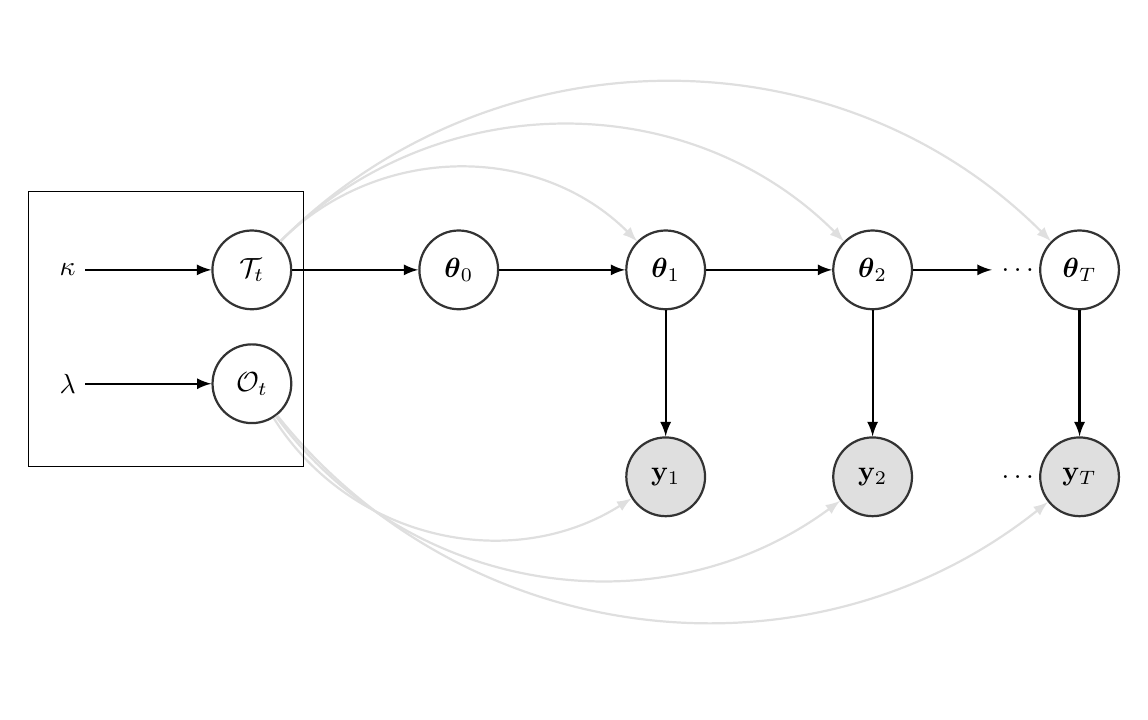
\begin{tikzpicture}
		\tikzstyle{main}=[circle, minimum size = 10mm, thick, draw =black!80, node distance = 16mm]
		\tikzstyle{connect}=[-latex, thick]
		%\tikzstyle{box}=[rectangle, draw=black!100]
		\node[ fill = white!100] (kappa) {$\kappa$};
		\node[main] (T) [right=of kappa] {$\mathcal{T}_t$};
		
		\node[] (lambda) [below=of kappa] {$\lambda$};
		\node[main] (O) [right=of lambda] {$\mathcal{O}_t$};
		
		\node[main] (theta0) [right=of T] {$\boldsymbol{\theta}_0$};
		\node[main] (theta1) [right=of theta0] {$\boldsymbol{\theta}_1$};
		\node[main] (theta2) [right=of theta1] {$\boldsymbol{\theta}_2$};
		\node[main] (thetaT) [right=of theta2] {$\boldsymbol{\theta}_T$};
		
		\node[main, fill = gray!25] (y1) [below=of theta1] {$\mathbf{y}_1$};
		\node[main, fill = gray!25] (y2) [right=of y1] {$\mathbf{y}_2$};
		\node[main, fill = gray!25] (yT) [right=of y2] {$\mathbf{y}_T$};
		
		
		\path (kappa) edge [connect] (T);
		\path (lambda) edge [connect] (O);
		
		\path (T) edge [connect] (theta0);
		
		\path (theta0) edge [connect] (theta1);
		\path (theta1) edge [connect] (theta2);
		
		\path (theta1) edge [connect] (y1);
		\path (theta2) edge [connect] (y2);
		\path (thetaT) edge [connect] (yT);
		
		\node[] (dots) [right=of theta2]{\ldots};
		\node[] (dotsy) [right=of y2]{\ldots};
		
		\path (theta2) edge [connect] (dots);
		
		\path[bend right=45, color = gray!25] (O) edge [connect] (y1);
		\path[bend right=45, color = gray!25] (O) edge [connect] (y2);
		\path[bend right=45, color = gray!25] (O) edge [connect] (yT);
		
		\path[bend left=45, color = gray!25] (T) edge [connect] (theta1);
		\path[bend left=45, color = gray!25] (T) edge [connect] (theta2);
		\path[bend left=45, color = gray!25] (T) edge [connect] (thetaT);
		
		\draw[] (-0.5,-2.5) rectangle (3,1);
		
	\end{tikzpicture}
\caption{Visualization of the eSIR model.}
\end{figure}

Regarding the function $f(\cdot)$, it is the solution to the dynamic system
%
\begin{equation}\label{eSIR}
	\frac{d\theta_t^S}{dt} = -\rho\pi(t)\theta_t^S\theta_t^I, \quad \frac{d\theta_t^I}{dt} = \rho\pi(t)\theta_t^S\theta_t^I - \gamma \theta_t^I, \quad \frac{d\theta_t^R}{dt} = \gamma \theta_t^I,
\end{equation}
%
where the term $\pi(t)$ is a transmission modifier equal to $\pi(t) = (1-q^S(t))(1-q^I(t))$, where $q^S(t)$ denotes the probability of a susceptible person being in-home isolation, and $q^I(t)$ the probability of an infected person being in-hospital quarantine. The term $\pi(t)$ therefore is a transmission modifier in the sense that it modifies the probability of a susceptible person getting in contact with an infected person. The chance of such a meeting to occur is to a great extent determined by which restrictions on social gatherings are in place. For example, if a geographical region does not impose a quarantine, $\pi(t)=1$, and the dynamic system in (\ref{eSIR}) reduces to the classic formulation of the SIR model. As the rules of social distancing gets stricter, the transmission modifier $\pi(t)$ decreases, making the overall transmission rate to decrease as well. In this work, the $\pi(t)$ term is allowed to differ from 1. 

Since there are no explicit solutions available to (\ref{eSIR}), the so-called fourth-order Runge-Kutta approximation is implemented, meaning that 
%
$$
\begin{aligned}
	\begin{pmatrix}
		f(\theta_{t-1}^S) \\
		f(\theta_{t-1}^I) \\
		f(\theta_{t-1}^R)
	\end{pmatrix}
\end{aligned} = 
%
\begin{aligned}
	\begin{pmatrix}
		\theta_{t-1}^S + 1/6[k_{t-1}^{\theta^S_1} + 2k_{t-1}^{\theta^S_2} + 2k_{t-1}^{\theta^S_3} + k_{t-1}^{\theta^S_4}] \\
		\theta_{t-1}^I + 1/6[k_{t-1}^{\theta^I_1} + 2k_{t-1}^{\theta^I_2} + 2k_{t-1}^{\theta^I_3} + k_{t-1}^{\theta^I_4}] \\
		\theta_{t-1}^R + 1/6[k_{t-1}^{\theta^R_1} + 2k_{t-1}^{\theta^R_2} + 2k_{t-1}^{\theta^R_3} + k_{t-1}^{\theta^R_4}]
	\end{pmatrix}
\end{aligned}
$$
%
where 
%
\begin{equation*}
\begin{split}	
		k_{t-1}^{\theta^S_1} &= - \rho\pi(t-1) \theta_{t-1}^S \theta_{t-1}^I, \\
		%
		k_{t-1}^{\theta^S_2} &= - \rho\pi(t-1) [\theta_{t-1}^S + 0.5 k_{t-1}^{\theta^S_1}] [\theta_{t-1}^I + 0.5 k_{t-1}^{\theta^I_1}], \\
		%
		k_{t-1}^{\theta^S_3} &= \rho\pi(t-1) [\theta_{t-1}^S + 0.5 k_{t-1}^{\theta^S_2}] [\theta_{t-1}^I + 0.5 k_{t-1}^{\theta^I_2}], \\
		%
		k_{t-1}^{\theta^S_4} &= \rho\pi(t-1) [\theta_{t-1}^S + k_{t-1}^{\theta^S_3}] [\theta_{t-1}^I + k_{t-1}^{\theta^I_3}],
\end{split}
\end{equation*}
%
\begin{equation*}
	\begin{split}	
		k_{t-1}^{\theta^I_1} &= \rho\pi(t-1) \theta_{t-1}^S \theta_{t-1}^I - \gamma \theta^I_{t-1}, \\
		%
		k_{t-1}^{\theta^I_2} &= \rho\pi(t-1) [\theta_{t-1}^S + 0.5 k_{t-1}^{\theta^S_1}] [\theta_{t-1}^I + 0.5 k_{t-1}^{\theta^I_1}] - \gamma[\theta_{t-1}^I + 0.5 k_{t-1}^{\theta^I_1}], \\
		%
		k_{t-1}^{\theta^I_3} &= \rho\pi(t-1) [\theta_{t-1}^S + 0.5 k_{t-1}^{\theta^S_2}] [\theta_{t-1}^I + 0.5 k_{t-1}^{\theta^I_2}] - \gamma[\theta_{t-1}^I + 0.5 k_{t-1}^{\theta^I_2}], \\
		%
		k_{t-1}^{\theta^I_4} &= \rho\pi(t-1) [\theta_{t-1}^S + k_{t-1}^{\theta^S_3}] [\theta_{t-1}^I + k_{t-1}^{\theta^I_3}] - \gamma[\theta_{t-1}^I + k_{t-1}^{\theta^I_3}], 
	\end{split}
\end{equation*}
%
and 
%
\begin{equation*}
	\begin{split}	
		k_{t-1}^{\theta^R_1} &= \gamma \theta^I_{t-1}, \\
		%
		k_{t-1}^{\theta^R_2} &= \gamma[\theta_{t-1}^I + 0.5 k_{t-1}^{\theta^I_1}], \\
		%
		k_{t-1}^{\theta^R_3} &= \gamma[\theta_{t-1}^I + 0.5 k_{t-1}^{\theta^I_2}], \\
		%
		k_{t-1}^{\theta^R_4} &= \gamma[\theta_{t-1}^I + k_{t-1}^{\theta^I_3}]. 
	\end{split}
\end{equation*}
%	



%\begin{tikzcd}[nodes in empty cells]
%	\text{Markov process:}
%	&   \boldsymbol{\theta}_0
%	&   \boldsymbol{\theta}_1 \ar[dd]
%	&   \boldsymbol{\theta}_2  \ar[dd]
%	&   \dots  
%	&   \boldsymbol{\theta}_{T-1} \ar[dd]       \\
%	&   \arrow[rrrr, dashed, -,
%	start anchor={[shift={(-3ex,2ex)}]north west},
%	end anchor  ={[shift={( 3ex,2ex)}]north east}]
%	&   &   &   &   &                               \\
%	\text{Observations:}
%	&   \mathbf{y}_0
%	&   \mathbf{y}_1
%	&   \mathbf{y}_2
%	&   \dotsm
%	&   \mathbf{y}_{T-1}           \\
%\end{tikzcd}



\section{The State-Space Latent Block Model}
Both the SIR model and the eSIR model assume that the population of cases are freely mixed in the population, although in many real situations the mixing of a specific group of cases might have geographical limitations. Moreover, although the eSIR allows for a varying transmission rate $\rho$, the modifier function $\phi(t)$ needs to be defined by the modeler. With a pandemic like the 2020 coronavirus, the modifier function would furthermore differ between different geographical regions. With the aim to increase predictive accuracy, we address these issues by incorporating into the eSIR model a latent block model component, presented in the following. The general idea is to simultaneously identify row clusters of geographical regions and column clusters of time points in the data matrix $\mathbf{y}$, and then re-define the eSIR model on these identified block clusters. In this way we will both be able to make forecasts on geographical regions identified by the row clusters, and estimate the transmission modifier $\pi(t)$ with data by setting it according to the estimated column clusters.
 
With $n$ geographical regions measured on $T$ time points, the data matrix $\mathbf{y}$ that we wish to co-cluster equals
%
$$
\mathbf{y} = \begin{bmatrix}
	(y^I_1(1), y^R_1(1)) & (y^I_1(2), y^R_1(2)) & \ldots & (y^I_1(T), y^R_1(T))\\
	(y^I_2(1), y^R_2(1)) & (y^I_2(2), y^R_2(2)) & \ldots & (y^I_2(T), y^R_2(T))\\
	\vdots & \vdots & \ldots & \vdots \\
	(y^I_n(1), y^R_n(1)) & (y^I_n(2), y^R_n(2)) & \ldots & (y^I_n(T), y^R_n(T))
\end{bmatrix}
$$
%
Following the latent block model, we assume that there is a partition ($Z, W$) of the data matrix $\mathbf{y}$, where $Z = (z_{ik}; , i=1,\ldots, n, \: k = 1,\ldots, K)$ represents the partitioning into $K$ clusters on the $n$ rows and $W = (w_{tl}; t=1,\ldots, T, \: l=1,\ldots, L)$ represents the partitioning into $L$ clusters on the $T$ measured time-points (columns). In other words, $Z_{ik}$, $k = 1,..., K$ and $W_{tl}$, $l = 1,..., L$ are binary matrices for which $Z_{ik} = 1$ if case $i$ belongs to row cluster $k$ and $0$ otherwise, and $W_{tl} = 1$ if time point $t$ belongs to column cluster $l$ and $0$ otherwise. The random matrices $Z$ and $W$ therefore are of dimension $n \times K$ and $T \times L$, respectively. 

Co-clustering will yield subgroups, called blocks, such that $Z_{ik} W_{tl} = 1$. Each element $\mathbf{y}_{i}(t)$ in $\mathbf{y}$ belongs to a block which is generated by a probability distribution. In this study it is assumed that $y_{i}^I(t)$ and $y_{i}^R(t)$ follow Beta distributions, meaning that these block distributions are given by the distributions specified by Equation \ref{statespace}. Specifically, we assume that for a geographical region $i$ belonging to row cluster $k$ and a time-point $t$ belonging to column cluster $l$, the block $Z_{ik}W_{jl}$ is generated by the following distributions: 
%
\begin{equation}\label{statespace-observed}
	\begin{aligned}
		y_{i}^I | Z_{ik}W_{jl} = 1, \boldsymbol{\Omega}_1 \sim \text{Beta}(\lambda^I \theta_{kl}^I, \lambda^I(1 - \theta_{kl}^I) \\
		%
		y_{i}^R | Z_{ik}W_{jl} = 1, \boldsymbol{\Omega}_1 \sim \text{Beta}(\lambda^R \theta_{kl}^R, \lambda^R(1 - \theta_{kl}^R)
	\end{aligned}
\end{equation}
% 
%and 
%
%\begin{equation}\label{statespace-latent}
%	\boldsymbol{\theta}_t | \boldsymbol{\theta}_{t-1}, \boldsymbol{\Omega}_1 \sim \text{Dirichlet}(\kappa f(\boldsymbol{\theta}_{kl}(t-1)))
%\end{equation}
%
where  
%
$
\theta_{kl}^I
$
%
and 
%
$
\theta_{kl}^R
$
%
denote the probabilities of a case in row cluster $k$ and column cluster $l$ being infected and removed, respectively. Regarding the state process, we are going to deviate from the eSIR model and the Dirichlet distribution. The reason is that $\theta_{kl}$ is now guiding the observed data, and the time clusters are allowed to re-appear in the time interval. To illustrate that idea, consider Figure \ref{timeline}. We have, by co-clustering the data matrix using the LBM, ended up with three time (column) clusters. To illustrate how these clusters spread out across time, we 

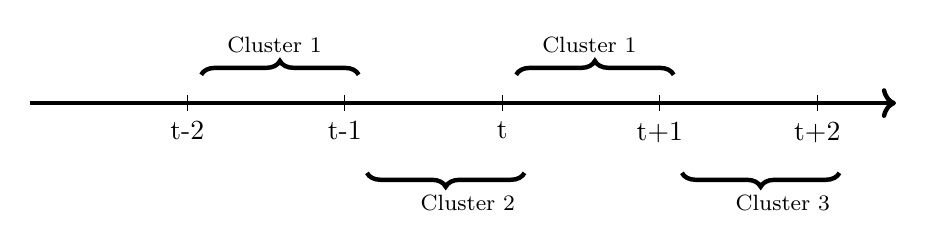
\begin{tikzpicture}\label{timeline}
	% draw horizontal line   
	\draw[ultra thick, ->] (0,0) -- (\ImageWidth,0);
	
	% draw vertical lines
	\foreach \x in {2,4,6,8,10}
	\draw (\x cm,3pt) -- (\x cm,-3pt);
	
	% draw node
	\draw[ultra thick] (2,0) node[below=3pt,thick] {t-2} node[above=3pt] {};
	\draw[ultra thick] (4,0) node[below=3pt,thick] {t-1} node[above=3pt] {};
	\draw[ultra thick] (6,0) node[below=3pt, thick] {t} node[above=3pt] {};
	\draw[ultra thick] (8,0) node[below=3pt] {t+1} node[above=3pt] {};
	\draw[ultra thick] (10,0) node[below=3pt] {t+2} node[above=3pt] {};
	
	\draw [black, ultra thick ,decorate,decoration={brace,amplitude=5pt},
	xshift=5pt,yshift=-4pt] (2,0.5)  -- (4,0.5) 
	node [black,midway,above=4pt,xshift=-2pt] {\footnotesize Cluster 1};
	
	\draw [ black, ultra thick,decorate,decoration={brace,amplitude=5pt},
	xshift=8pt,yshift=-11pt] (6,-0.5) -- (4,-0.5)
	node [black,midway,below=4pt,xshift=8pt] {\footnotesize Cluster 2};
	
	\draw [ black, ultra thick,decorate,decoration={brace,amplitude=5pt},
	xshift=5pt,yshift=-4pt] (6,0.5) -- (8,0.5)
	node [black,midway,above=4pt,xshift=-2pt] {\footnotesize Cluster 1};
	
	\draw [ black, ultra thick,decorate,decoration={brace,amplitude=5pt},
	xshift=8pt,yshift=-11pt] (10,-0.5) -- (8,-0.5)
	node [black,midway,below=4pt,xshift=8pt] {\footnotesize Cluster 3};
	
\end{tikzpicture}

According to the figure, the first time (column) cluster equals the time period between $t-2$ and $t-1$. The next period of time, between $t-1$ and $t$ belongs to cluster 2, and after that we are back at cluster 1 before entering cluster 3. The LBM offers us the flexibility to return to clusters as we progress in time. This property seems well-suited when modeling the coronavirus pandemic as we for example currently are seeing a widespread second wave hit many countries. 

To model the transition between time clusters, we need to estimate the transition matrix $A = [a_{l, l^\prime}]$, 
%
$
[a_{l, l^\prime}] = P(\boldsymbol{\theta} = \boldsymbol{\theta}_{kl^\prime} |\boldsymbol{\theta} = \boldsymbol{\theta}_{kl} ). 
$
%
So for each row cluster $k$ we have a hidden Markov model with a latent process $\boldsymbol{\theta}_{kl}$ that guides the observed data $y_{kl}$. This means that we have in total $K$ HMMs, meaning a hidden Markov mixture model. Our set of observations are therefore samples from a groups of $K$ HMMs, each associated with a specific sub-behavior. 



We thus assume that the latent process $\boldsymbol{\theta}(t)$ guides the observed data in each block cluster, that in turn is distributed according to a Beta distribution. 

It is assumed that $Z$ and $W$ are independent from each other and that the random variables $\mathbf{y}$ are independent conditional on $Z$ and $W$. With this formulation of the model we further assume that there is a partition of geographical regions that are homogeneous in terms of proportion infected $y^I(t)$ and removed $y^R(t)$, and that there is a partitioning of the time points $t$ that form homogeneous blocks.

Now let $\alpha_k = P(Z_{ik} = 1)$ and $\beta_l = P(W_{jl} = 1)$ denote the respective row and column mixing proportions such that they both sum to 1 and 
%
$
p(z; \theta) = \prod_{ik} \alpha_k^{z_{ik}} 
$
%
and 
%
$
p(w; \theta) = \prod_{ik} \beta_l^{w_{jl}}. 
$ 
%
Under the assumption of $Z$ and $W$ being independent, and by letting $\mathcal{Z}$ and $\mathcal{W}$ denote the sets of all possible partitions of $Z$ and $W$, the likelihood of the LBM equals
$$
L(\boldsymbol{\Omega}_2) = \sum_{(z, w) \in \mathcal{Z}, \mathcal{W}} \prod_{i, g} \alpha^{z_{ig}} \prod_{j, l} \beta^{w_{jl}} \prod_{i, j, k, l} \varphi(\mathbf{y}_{ij}; \omega_{kl})^{z_{ig} w_{jl}},
$$
%
where $\omega_{kl}$ represents the parameter of $\varphi$ for the $kl$ block. The log-likelihood equals 
%
$$
\log L(\boldsymbol{\Omega}_2) = \sum_{i, k} z_{ik} \log\alpha_k \sum_{j, l} w_{jl} \log \beta_l \sum_{i, j, k, l} z_{ik} w_{jl} \log\varphi(\mathbf{y}_{ij}; \omega_{kl}),
$$
%

The state-space LBM can now graphically be represented as

\begin{figure}[H]
	\centering
	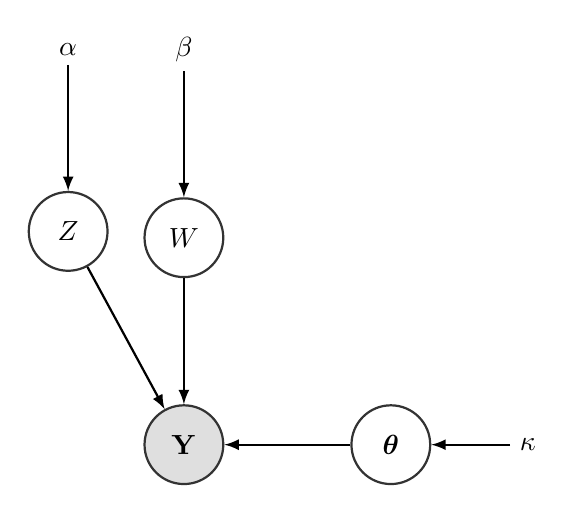
\begin{tikzpicture}
		\tikzstyle{main}=[circle, minimum size = 10mm, thick, draw =black!80, node distance = 16mm]
		\tikzstyle{connect}=[-latex, thick]
		%\tikzstyle{box}=[rectangle, draw=black!100]
		\node[ fill = white!100] (alpha) {$\alpha$};
		\node[main] (Z) [below=of alpha] {$Z$};
		
		\node[] (beta) [right=of alpha] {$\beta$};
		\node[main] (W) [below=of beta] {$W$};
		
		\node[main, fill = gray!25] (Y) [below=of W] {$\mathbf{Y}$};
		\node[main] (theta) [right=of Y] {$\boldsymbol{\theta}$};
		
		\node[] (kappa) [right=of theta] {$\kappa$};
		
		\path (Z) edge [connect] (Y);
		\path (W) edge [connect] (Y);
		
		\path (theta) edge [connect] (Y);
		
		\path (alpha) edge [connect] (Z);
		\path (beta) edge [connect] (W);
		
		\path (kappa) edge [connect] (theta);
		
		%\node[rectangle, inner sep=0mm, fit= (z) (w),label=below right:N, xshift=13mm] {};
		%\node[rectangle, inner sep=4.4mm,draw=black!100, fit= (z) (w)] {};
		%\node[rectangle, inner sep=4.6mm, fit= (z) (w),label=below right:M, xshift=12.5mm] {};
		%\node[rectangle, inner sep=9mm, draw=black!100, fit = (theta) (z) (w)] {};
	\end{tikzpicture}
\end{figure}	


\section{Estimation}

Since there are two model components of the eSIR LBM, we repeat the total set of parameters that needs to be estimated. The unknown parameters from the eSIR model component of the likelihood thus equals 
%
$ 
\boldsymbol{\Omega}_1 = (\rho, \gamma, \boldsymbol{\theta}, \lambda, \kappa)
$ 
%
and the LBM model component of the likelihood equals
%
$ 
\boldsymbol{\Omega}_2 = (\alpha, \beta, \omega).
$ 
%
The total set of parameters to be estimated thus equals 
%
$
\boldsymbol{\Omega} = \boldsymbol{\Omega}_1 + \boldsymbol{\Omega}_2 = (\rho, \gamma, \boldsymbol{\theta}, \lambda, \kappa, \alpha, \beta, \omega).
$
%

For the estimation of the eSIR LBM model, we will assume that $\varphi(\mathbf{y}_{ij}; \omega_{kl})$ follows a Dirichlet distribution:
%
$$
\varphi(\mathbf{y}_{ij}; \omega_{kl}) = D(\omega_{kl})^{-1} \prod_{j=1}^{d+1} y_{ij}^{\omega_{kl}-1}
$$
%
So should we model $\varphi(\cdot)$ as a bivariate beta distribution (meaning Dirichlet distribution)? Regarding this, see the paper "Time Series of Continuous Proportions", by Grunwald, Raftery and Guttorp (1993), where they model the time series of proportions using the Dirichlet distribution.


There is a paper ("Estimation and selection for the latent block model on categorical data" by Keribin et al.) that implements the LBM for multinomial data that in the estimation of the model sets prior distributions for the mixing proportions as well as the parameter that governs the $Y$ distribution. This would in a sense be similar to our case, since the eSIR model imposes a Dirichlet prior on the $\boldsymbol{\theta}$ parameter. If we would further impose Dirichlet priors on the mixing proportions, would we be able to do something similar as in Keribin et al.?

So specifically, following \parencite{keribin2015estimation} we can consider proper and non-informative priors for $\alpha$ and $\beta$ as
%
\begin{equation}
	\begin{aligned}
		\boldsymbol{\alpha} \sim \text{Dirichlet}(a, \ldots, a) \\
		%
		\boldsymbol{\beta} \sim \text{Dirichlet}(a, \ldots, a)
	\end{aligned}
\end{equation}
%

In \parencite{keribin2015estimation} they consider a very similar general modeling structure and estimate the model parameters $\boldsymbol{\tau}$ by maximizing the posterior density $p(\boldsymbol{\tau} | \boldsymbol{y})$, which leads to the Maximum A Posteriori (MAP) estimator: 
%
\begin{equation}
	\hat{\boldsymbol{\tau}}_{MAP} = \underset{\boldsymbol{\tau}}{\mathrm{argmax}} \: p(\boldsymbol{\tau} | \boldsymbol{y})
\end{equation}
 
We would thus be able to graphically represent the model as 
%
\begin{figure}[H]
	\centering
	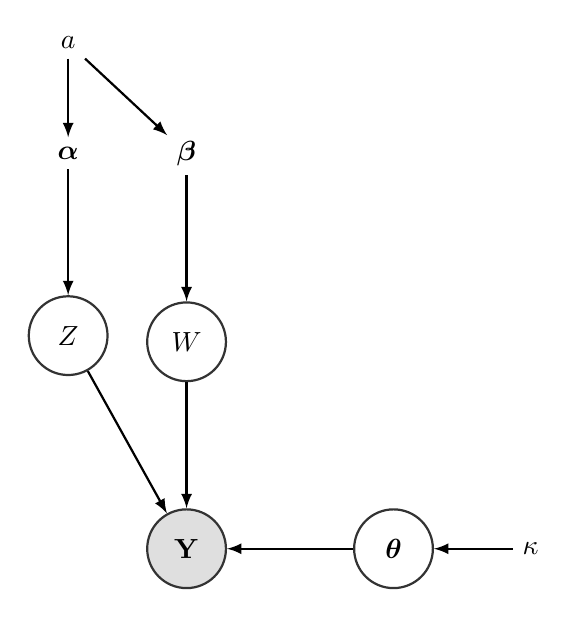
\begin{tikzpicture}
		\tikzstyle{main}=[circle, minimum size = 10mm, thick, draw =black!80, node distance = 16mm]
		\tikzstyle{connect}=[-latex, thick]
		%\tikzstyle{box}=[rectangle, draw=black!100]
		\node[ fill = white!100] (alpha) {$\boldsymbol{\alpha}$};
		\node[main] (Z) [below=of alpha] {$Z$};
		
		\node[] (a) [above= of alpha] {$a$}; 
		
		\node[] (beta) [right=of alpha] {$\boldsymbol{\beta}$};
		\node[main] (W) [below=of beta] {$W$};
		
		\node[main, fill = gray!25] (Y) [below=of W] {$\mathbf{Y}$};
		\node[main] (theta) [right=of Y] {$\boldsymbol{\theta}$};
		
		\node[] (kappa) [right=of theta] {$\kappa$};
		
		\path (Z) edge [connect] (Y);
		\path (W) edge [connect] (Y);
		
		\path (a) edge [connect] (alpha);
		\path (a) edge [connect] (beta);
		
		\path (theta) edge [connect] (Y);
		
		\path (alpha) edge [connect] (Z);
		\path (beta) edge [connect] (W);
		
		\path (kappa) edge [connect] (theta);

	\end{tikzpicture}
\end{figure}



\printbibliography

\end{document}